% dissertation.tex	K. J. Turner	10/09/13

% Dissertation outline

\documentclass[a4paper,11pt]{report}

\usepackage{dissertation}
\usepackage{identfirst}
\usepackage{graphicx}
\usepackage{chngcntr}
\counterwithout{figure}{chapter}

\title{Smart contracts on Hyperledger Fabric}			

\author{
{Yordan Gospodinov} \\
{\small{Supervised by Dr. Andrea Bracciali}}
}

\renewcommand{\baselinestretch}{1.1}
\date{April 2019}			

\degree{B. Sc. in Computer Science}

\begin{document}

\maketitle				

\pagenumbering{roman}


%%%%%%%%%%%%%%%%%%%%%%%%%%%%%%%%%%  Abstract %%%%%%%%%%%%%%%%%%%%%%%%%%%%%%%%%%%

\intro{Abstract}

Summarise the dissertation within one page. Introductory headings like this are
entered using the {\it intro} paragraph style. It is suggested that the abstract
be structured as follows:

\begin{description}

  \item[Problem:]
  what you tackled, and why this needed a solution

  \item[Objectives:]
  what you set out to achieve, and how this addressed the problem

  \item[Methodology:]
  how you went about solving the problem

  \item[Achievements:]
  what you managed to achieve, and how far it meets your objectives.

\end{description}


%%%%%%%%%%%%%%%%%%%%%%%%%%%%%%%%%  Attestation %%%%%%%%%%%%%%%%%%%%%%%%%%%%%%%%%

\intro{Attestation}

I understand the nature of plagiarism, and am aware of the University's policy
on this. I certify that this dissertation reports original work by me during my
University project except for the following (adjust according to the
circumstances):

\begin{itemize}

  \item
  The technology review in section~\ref{technical-section2} was largely adapted
  %from \cite{Greene-Williams-1997} plus
  \url{www.software-review.org/article9815.html}.

  \item
  The code discussed in section~\ref{technical-section1} was created by Acme
  Corporation (\url{www.acme-corp.com/JavaExpert}) and was used in accordance
  with the licence supplied.

  \item
  The code discussed in section~\ref{technical-subsection1} was written by my
  supervisor.

  \item
  The code discussed in section~\ref{technical-subsubsection2} was developed by
  me during a vacation placement with the collaborating company. In addition,
  this used ideas I had already developed in my own time.

\end{itemize}

\bigskip

{\bf Signature:} \hspace{20em} {\bf Date:}


%%%%%%%%%%%%%%%%%%%%%%%%%%%%%%%  Acknowledgements %%%%%%%%%%%%%%%%%%%%%%%%%%%%%%

\intro{Acknowledgements}

First and foremost I would like to thank to Dr. Andrea Bracciali for introducing me to blockchain. What's more I am grateful for his patience, guidance and support, without which I would not have been able to grow into what I am today. Thank you.

I am grateful to my parents for giving me the opportunity to study in University of Stirling. 

I am grateful to my classmates for helping me out, when I could not understand something, and just for being around, it was fun. 

I would like to thank the library for having the nice, quiet, fourth floor, and for always buying the books I requested. 

%%%%%%%%%%%%%%%%%%%%%%%%%%%%%%%%%%  Contents %%%%%%%%%%%%%%%%%%%%%%%%%%%%%%%%%%%

\tableofcontents

\listoffigures                

% \listoftables                 

\clearpage

\pagenumbering{arabic}

\setcounter{page}{1}


%%%%%%%%%%%%%%%%%%%%%%%%%%%%%%%%  Introduction %%%%%%%%%%%%%%%%%%%%%%%%%%%%%%%%%

\chapter{Introduction}

\label{introduction}

Recently a new technology emerged into the world that is called blockchain. The idea is that it is a distributed decentralized database of blocks of transactions. The reason why I find it so interesting is that it has the potential to change many aspects of life, by changing the way of accessibility and security of a data. Hyperledger Fabric is a blockchain framework designed especially to make the system easily adoptable for different business use cases. The main two objectives of this project are: to research how the smart contracts in Hyperledger Fabric works; to make a prototype of self-sovereign system with the gathered knowledge. 

\section{Background and Context}

\label{introduction-background}

Information has always been one of the most valuable assets a person could have. Through times information was traded in many different ways, from barter to monetization. Recently the information about an individual has become a great selling point, because it can be used in variety of fields, from science to business. However, the collection of this data is becoming a problem.

	As individuals, our identities are, to some extend, not ours anymore. If we cannot certify who we are, we became no one in the eyes of business and government. Needless to say that have we lost all of the documents that certify our place in the city, company, country, Earth, we would be in a big trouble. \cite{allen2016path}
	
		Another approach to critical and private information is how it is being used live. Whenever we want to identify ourselves somewhere, the usual document for identification would be either an ID or a passport. Here is the problem concerning all information on this document. It turns out that whenever a person wants to prove his or her existence, the party that requires this identification, can take and keep a record of all sensitive data on that document. In some countries this may be illegal. This data then could be used for not a rightful purpose. \cite{alboaie2017private}
		
Furthermore whenever a person is signing in to receive some kind of certificate, whether that would be a school or an academy, he or she is leaving sensitive data with this company. In most countries, whenever a person starts living in a city, he or she has to identify himself/herself to the council. In the end, there is a lot of institutions that keep sensitive data for an individual. This is a problem, because some of those institutions or businesses have different levels of security. So, an attacker only needs to pick the easiest target, and he will get a great deal of sensitive data. 

	I believe all of these problems are just a subproblems of a bigger challenges - what is an identity today and how to be able to give private access to our data. The solution could provide us awareness for a better control of our own data, as well as to be able to share only what’s exactly needed to provide to those companies and institutions.

\subsection{Distributed Ledger Technologies}

\label{dlt}

Ledgers have been in use of the humanity since ancient days. Their medium has been clay, wooden tally sticks, stone, papyrus and paper. They served its purpose as a one-side record-keeping tool. But this also brings concerns around who is going to validate this one-side register. Later in 15th century, the Italian mathematician Luca Pacioli became the first person, recorded, to publish a paper on the double-entry bookkeeping \cite{ledgers}.However, even when all of the parties have their own records of a particular deal, someone, or even a group of the participants, may cheat and keep a different record, from the original. Thus taking advantage over the people who are trying to trade fairly and honorably.

However, even when all of the parties have their own records of a particular deal, someone, or even a group of the participants, may cheat and keep a different record, from the original. Thus taking advantage over the people who are trying to trade fairly and honorably.

A distributed ledger technology is a concurrent system, referring to a database that is consistently shared and synchronized across multiple machines/nodes in a network. It allows transactions to be monitored by multiple actors, thereby making a cyberattack more difficult. The participants at each of those machines can access the recordings shared and can keep an identical copy of it. Since it is a distributed ledger, any changes made on it are then reflected and the change is done to all the nodes holding a copy of it \cite{dltref} . However, in order to know which entry should be spread, and which is/are the correct ledger/s the system has to have a consensus among all the peers and reach a final solution.
\subsubsection{Cosensus}  
\label{consensus}

In general, a consensus algorithm is a process in computer science used to achieve agreement on a single data value among distributed processes or systems. Consensus algorithms are designed to achieve reliability in a network involving multiple unreliable nodes. Solving that issue – known as the consensus problem – is important in distributed computing and multi-agent systems.\cite{mills2016distributed}
\subsubsection{Cross-border transactions}  
\label{xborderTransactions}

Includes both outbound and inbound transfers of property, stock, or financial and commercial obligations between related entities resident or operating in different tax jurisdictions. Until recently developers argued that certain attributes of DLT, such as the ability to share ledgers across geographic distances and time-zones, could reduce the number of intermediaries needed to effect cross-border payments. Cross-border payments may be a product of a more transparent and cost-efficient structure due to reducing the number of intermediaries. As result of the reduction, a certain regional banks may be able to directly access the network, thus resulting in the benefits mentioned.\cite{mills2016distributed}


\subsubsection{Information Sharing}  
\label{infosharing}
DLT has the ability to maintain tamper-resistant records and the arrangements could be designed to allow participants to have “read-only access” to certain parts of the common ledger. This even if it limits the user’s options, it still gives visibility which in turn stresses the integrity of the system, since you are being able to see the supply chain of a particular asset or its history. At the same time, however, since not all of a service provider’s transactions concerning customers might be on one or more ledgers, certain regulatory requirements could be difficult to meet by simply providing access to a ledger.\cite{mills2016distributed}

\subsection{Blockchain}
\label{blockchain}

Blockchain is a new technology that represents several ideas that are now able to work together. In its core, this high tech is decentralized database. Moreover, due to the asymmetric (public - private key ) cryptography, every peer has an unique identity. Whenever a peer adds data into the blockchain, everybody in the network can see his or her public address as an initiator of this transaction. Since everyone participates in this database, no duplication of data is made, hence no redundancy. 

In the blockchain each block’s header includes a hash of the block’s transactions, as well as a copy of the hash of the prior block’s header, hence blockchain. In this way, all transactions are sequenced and cryptographically linked together. This mechanism keeps the ledger data very secure. Even if one node hosting the ledger has been tampered with, it would not be able to convince all the other nodes that it has the ‘correct’ data, because the ledger is distributed through a network of independent nodes. [Fabric ledger doc] 
 
	Blockchain is a linked list of blocks and a block is a group of ordered transactions. It is a distributed database on which once a data has been put, that data cannot be changed. Another unique feature is that there are specific rules, which can put data into the block. These rules, protocol, are made so that there could be no conflicts with data that is already in the database. The data is locked on to an owner. Finally, the nodes agree upon the state of the blockchain.\cite{whatIsBlockchain} It is important that in different blockchains the consensus can be different as well. Thus, two blockchains can have different unique features.
	
	An important notion is that a blockchain network can be \textit{permissioned} or \textit{permissionless}.

\subsubsection{Permissioned blockchain}
This type of network means that only the ones with permission can enter the network. The consensus can be more or less a variation of “Proof-of-authority”, where selected nodes endorse and agree between each other of the state of the blockchain. In this case, the trade off is that the system is not as decentralized, however the transactions are much faster and cost-effective.

\subsubsection{Permissionless blockchain}
Everyone can join in the network. Perfect examples of such systems are Bitcoin and Ethereum. Typically the consensus they execute at the moment is called “Proof-of-Work”. This mechanism allows every node to participate in a fair contest to ‘mine’ the next block. The winner gets either Bitcoin or Ether respective to the network. This type of consensus and availability to enter the network is giving the blockchain its most famous feature - being decentralized.

\subsubsection{Cryptocurrency}
Cryptocurrency is a digital asset, medium of exchange in the network. It is created and stored electronically in the blockchain by using encryption techniques to control the creation of monetary units and to verify the transfer of funds. The most important features that cryptocurrency possess are: it has no intrinsic value - you cannot redeem it for a raw material; it has no physical form; its supply is not determined by anyone but the creators of the respective blockchain. \cite{whatIsCryptocurrency}
An example of a working blockchain system with a cryptocurrency can be seen on figure \ref{blockchainAbstract}. 


A peer makes a transaction. This transaction is then taken upon consideration whether it is valid or not. The decision is made by all nodes or just the ones that have been given permission to validate transactions. Upon reaching the conclusion that a transaction is valid,  then it is wrapped up with many more, or in some cases alone, in order to create a block. Two things happen from the last event. First, a transaction is being completed. Second, in permissionless blockchains, the one to win the competition, to ‘mine’ the newly created block receives a reward. 

\begin{figure}[h]
\centering
  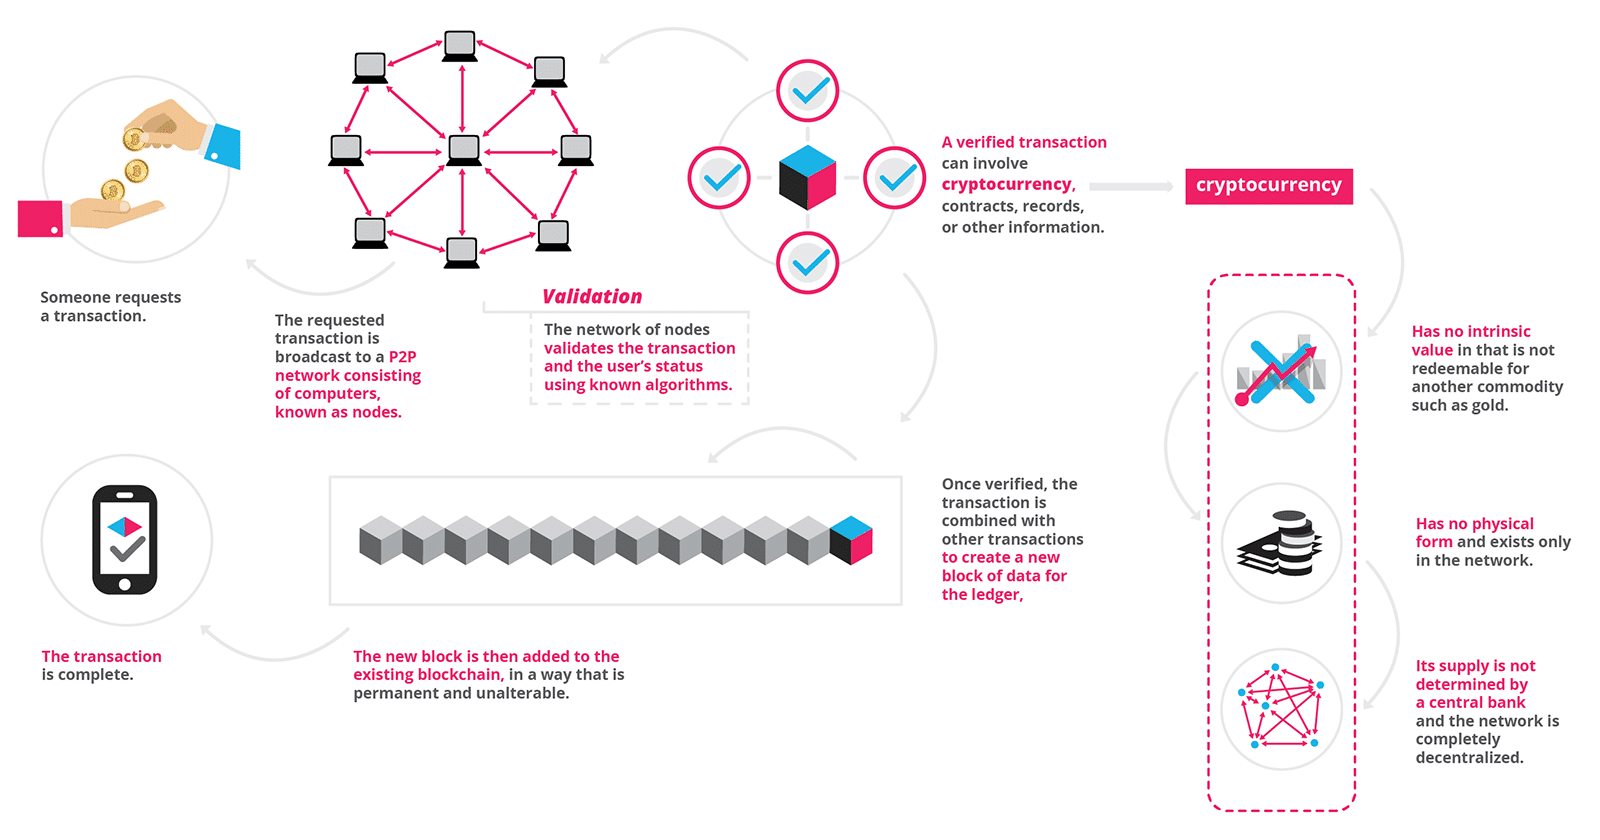
\includegraphics[width=16cm]{infographics0517-01-1.png}
  \caption{An abstract of a blockchain system \cite{whatIsBlockgeeks}}
  \label{blockchainAbstract}
\end{figure}



\section{Scope and Objectives}

\label{introduction-objectives}

The scope will involve Blockchain technology and what is digital identity. This project will focus on Hyperledger Fabric. This is a permissionless blockchain modular framework, especially developed for businesses.
 
Being a modular framework, a lot of the scope will involve around resolving how customizable Fabric can be. To be personalized is of an essence for the creation of a good system. The other main features to be examined are the scalability and usability of this blockchain framework.   

The knowledge build up from the research will be implemented in a prototype program as a final part of the project. The prototype of the self-sovereign program will focus on the decentralized nature. This work will aim to present advantages of the decentralizing element that can save resources and protect the personal data of the end-user. Last but not least, I am going to talk about how the ledger is making the whole system trustful, thus no one of the parties needs to worry about being cheated. 
 	
The objectives of the project include the following :  
\begin{itemize}
\item Understanding how Hyperledger Fabric work;
	\begin{itemize}
	\item Installing all prerequisites;
	\item Installing Hyperledger Fabric; 
	\item Running a simple network with 2 organizations; 
	\item Learning how to add more parties into an already running system;
	\item Trying out how the chaincode (smart contracts) work;
	\item Trying to install and control newly added chaincode on a running system.
	\end{itemize}
\item Building a fully functional Fabric blockchain with several different parties;
\item What an ID is  and identity and how it is defined in the digital world;
\item Deeper understanding of self-sovereign identity, what it is and how it should/could be best defined in a blockchain platform in order to be used genuinely and without misappropriation;
	\begin{itemize}
	\item Trying out different configurations on Fabric;
	\item Trying out different chaincode functions, to find out the best for the use case.
	\end{itemize}
\item Building a prototype of self-sovereign identity system ;
\item Complete final report .

\end{itemize}


\section{Achievements}

\label{introduction-achievements}

Summarise what you have achieved.

\section{Overview of Dissertation}

Briefly overview the contents of what follows in the dissertation.


%%%%%%%%%%%%%%%%%%%%%%%%%%%%%%  State-of-The-Art %%%%%%%%%%%%%%%%%%%%%%%%%%%%%%%

\chapter{State-of-The-Art}

\label{state}
\section{Successful projects made with Hyperledger Fabric}
\label{successfulFabric}

\subsection{Altoros}
\label{altoros}
Altoros is a software company that delivers different solutions. One of the problems their customers have is issuing bonds. The customer, Russia's National Settlement Depository (NSD), wanted a system that allows automate bond placement and accounting with blockchain, while minimizing risks of reconciliation and ensuring transparency. The reason they chose Fabric is for its support of confidential transactions and resilience in the production environment. \cite{altoros}

	What they did was to customize Fabric as needed for the different roles and actions. They set up four different channels so the communication,data transferring, between the peers and the NSD could be safe and secure. Every channel has its own chaincode ( smart contract) that is basically the logistics behind the given channel.
	
	One of the challenges they had was that the REST API was still in development. Fortunately, this is not the case anymore. Another challenge is that Fabric does not support cross-channel transactions. \cite{altorosDemo}
	
	The benefits of choosing Fabric are: 
	\begin{itemize}
	
\item Faster transactions compared to the traditional solution, where a lot of data exchanging has to be done through a middleman. Thus, not only making it faster but also cheaper. 
\item Minimizing fraud in a secure trusted network. The permissioned feature does not allow for anyone that does not meet the requirements to monitor what’s happening into the world ledger. What’s more because of the non cross-channel transactions, a peer could observe only the channels he is using. And even when he or she is inspecting another peer’s transaction, because of the encryption, he or she would not get any valuable information. 
\item Reduces expenses of the bond issuer by making the process faster and simplified
	\end{itemize}

\subsection{Verify.Me}
\label{verifyMe}
SecureKey is a company providing identity and authentication provider for simplified access to online services and applications. They are using trusted providers such as banks, telcos and governments to make their clients assert identity information and connect to critical online services with digital credentials.

After the government of Canada recognized their problem sending private data to a citizen, they asked for a solution. SecureKey responded to this call in collaboration with IBM with a blockchain based solution. It is a mobile app, that allows the user to connect different types of services providing only specific data. So what happens is the user connects to the blockchain through the phone. Then, it connects with the service actors. It is important to note that in the phone there are only pointers to the data and not the data itself. Whenever a person is sharing his or her identity with the new service he or she can see exactly what information is asked to be provided. \cite{verifyMe}

	The SIM card is used as an anchor of trust. Since the system is
private and permissioned blockchain, only trusted actors like banks and government can write on it. Upon losing or breaking the phone, the creators reassure that is easy to recover what’s lost. 
Again, here one of the main reasons to choose Fabric for the development of this service is mainly - the adaptability of the platform and the zero-knowledge proof supported concept. \cite{verifyMeDemo}

The benefits of using Fabric are : 
\begin{itemize}
\item Data integrity 
\item Security and resiliency
\item No central database or honeypots 
\item No central point of failure
\item Cannot track user across relying parties; privacy of the data
\item Cost efficient due to simplifying the process
\end{itemize}
Cons: 
\begin{itemize}
\item New - open standards needed 
\end{itemize}

\subsection{TradeLens}
\label{tradelens}

	TradeLens is a company founded by collaborative work of Maersk and IBM. Maersk is an integrated container logistics company working on improving the supply chain area. The idea is to make the shipping process cost-efficient, faster and in respect to accessing the needed documents - simpler.
	 
	For this task, the collaboration is combining their technical and specialized knowledge to build a system on top of Hyperledger Fabric. What they created is a network, that tracks the supply chain - the documents needed for starting a shipping process, the deal that is made, the location of the containers.
	 
	To participate, a user has to pay a price to enter the network. Still it is not confirmed what the requirements are. However, once a user decides to enter he will experience something way different from the usual way of things. Due to the blockchain technology, a user can check a block on the blockchain to track the location of the container or any other process involved. The usual way for this simple task would be to request this information from a middleman. TradeLens are saying they can reduce the paperwork and the need of a mediators, saving lots of time and money in the process. \cite{tradeLensFounders}
	
	It is important to be mentioned that TradeLens is not fighting the frauds. If a user input false data at start,that seems to be correct to the endorsement parties, the system won’t be able to catch it. So the network helps to have less fraud, but it is more of a side effect rather than main function.
	
	Another great use of this system is that, according to the World Trade Organization, simplifying the supply chain will not only reduce costs, but also help developing countries to increase their export by more than 30\% . [16]
	
\subsection{BitNation}
\label{bitnation}


\subsection{E-Residency}
\label{eResidency}

%%%%%%%%%%%%%%%%%%%%%%%%%%%%%% Technical Chapters %%%%%%%%%%%%%%%%%%%%%%%%%%%%%%

\chapter{Technology required}            % Insert your chapter titles

\label{technical}

The key software and technology used for the creation and development of this project is:
\begin{itemize}
\item OS: Ubuntu 16.04 Xenial 64 bit
\item Hyperledger Fabric - modular blockchain framework
\item Hyperledger Composer - a tool to create abstract blockchain application, that can then be run on Fabric.
\item Docker and Docker Composer
\item Visual Studio Code
\end{itemize}


\section{Docker}
\label{docker}

\section{Visual Studio Code}
\label{vsCode}
%%%%%%%%%%%%%%%%%%%%%%%%%%%%%%%%%%  Fabric  %%%%%%%%%%%%%%%%%%%%%%%%%%%%%%%%%
\chapter{Hyperledger Fabric}
\label{hplFabric}

\subsubsection{Permissioned blockchain}
A blockchain where the peers need to meet certain requirements to enter the network where he or she can perform certain actions is called permissioned. These systems are more attractive for the business and enterprise because they are faster and more cost-effective. Another feature that is appealing for those clients is the role system. That way actors, that all of the companies trust, can be the endorsers, the ones to validate the transactions. The feature could also be used to classify different players into respective roles. Which can give a particular system a better clarification and simplicity around executing different tasks. 

	It is not as decentralized system as the permissionless blockchain, however the tradeoff is acceptable enough for businesses to prefer it. The processes of “Anti-Money Laundering” and “Know Your Customer” require that service providers can confirm a peer’s legal identity and give clearance to make a transaction. The adoption of these processes in permissionless blockchain would be wrong, since they can illuminate who this peer is, thus breaking the promised anonymity. On another note, a permissioned blockchain can have larger volume of transactions per given time compared to a public one. 
	
What’s more, many prefer permissioned blockchains for supply chain. Since only the peers inside the blockchain can see what is happening on the path of a material to its final destination. And the tracking data can travel much faster, due to the simplified verification and less peers. 

\subsubsection{Hyperledger}
Hyperledger is a group of open source projects focused around cross-industry distributed ledger technologies. Hosted by The Linux Foundation, collaborators include industry leaders in technology, finance, banking, supply chain management, manufacturing, and IoT.


\section{Fabric overview}
	Fabric is one of those open source projects. It is a modular distributed ledger, which makes it highly customizable and adaptable to a variety of ideas and restrictions. The main scope of this undergraduate project is to test how functional and useful Fabric can be in different business and science situations. Is it making some of the use cases in those fields cheaper and more secure?
	
The feature which makes Fabric the perfect choice is that it can create different communication channels between different peers. Some of those channels could be for contract making between a supplier and a buyer. If a supplier has a favourite customer, he or she may give an exclusive deal. However, if everyone see this exclusive deal, then the business of the supplier would break down. That’s why this exclusive deal could exist in a confidential channel, one that only the two of them can see. 

	This Hyperledger project is a preferred platform mainly because of its adaptability to different use cases. One interesting feature, and main reason for the self-sovereign use case, is that Fabric supports zero-knowledge proof (ZKP). What this means is that it allows a peer to assure itself in front of a verifier without having to show any private data. This gives authority to ZKP to offer anonymous authentication for clients in their transactions. \cite{li2018fppb}
	
	The act of communication between different peers from different organizations (or groups) is through channels. These channels can be public or confidential. The communication inside works based on the chaincode, the smart contract. All of the logistics and functionality of a new blockchain application is based on it’s smart contracts. That is why they are extremely important and main object of interest in this undergraduate project.
\section{Fabric's Nodes}
\label{fnodes}
Hyperledger Fabric is set by organizations that want to setup a consortium. Every organization is constructed by several type of peer nodes (or just peers). All that these peers require is appropriate configuration and cryptographic materials like certificate authority (CA) and endorsement policy.
\subsubsection{Committing peer node}
The normal peer node or just peer, is a vital part of the Fabric’s network. This node is holding instances of the ledger, thus they commit the new blocks when received. Usually in production, multiple peer nodes are created. This impose redundancy, but it also create a no-single point of failure for the system. 
\subsubsection{Endorsing peer}
A special kind of commiting peers. They are important in the transaction flow and the consensus. When transaction is processed for verification, the endorsing peers are taking it and simulate what can happen if the transaction is added to the ledger. For that purpose, endorsing peers also have an instance of the chaincode in order to run the transaction proposal. If the simulation went well, and there were no problems with the current state of the ledger, the endorsing peer signs the transaction as validated. The endorsement is done by the committer nodes against the endorsement policy, which is specified when the chaincode is deployed. That means that while some channels will require majority of endorsing peers to run the transaction proposal, other could be happy with just a single endorsing peer.

\subsubsection{Orderer node}
It is pivotal for the consensus mechanism and transaction flow. It is responsible for consistent Ledger state across the network. Once the endorsing peers are done with the validation of a transaction, they send it to the orderer node. The orderer node is taking all transactions and then puts them into order, then batches them into blocks. Thereafter, the block are sent to the commiting peers via the anchor nodes.

	The orderer node neither executes the chaincode nor holds a copy of the blockchain. However, the ordering service (multiple nodes) are implementing specific ordering algorithms to decide what to do with the responses given from the endorsing peers. More about them in the consensus section.
\subsubsection{Anchor peer}
The anchor peer is the connection of the organization with the network. If there is no anchor peer in the organization, then this organization cannot connect to any other organization. What’s more important, it is the link between the orderer node and the ledger inside the organisations. If there is no mechanism to send or receive transactions then the whole organisation will become obsolete. Thus having setup several anchor peers, just in case of some unfaithful crash, is the safe bet.  

\section{Fabric's Ledger}
\label{fabricLedger}
	Consists of two distinct, though related, parts - \textbf{world state} and  a \textbf{blockchain}.
	
\subsection{World state}
\label{ws}
The world state is a database that holds the current values of the assets in the ledger as ledger states. The ledger states are usually expressed as key-value pairs, though there is some flexibility in this regard. The world state changes frequently because of the CRUD operations applied on the network. Needless to say, only validated transactions are able to change the ledger.

The world state is created with the premise of faster transactions. Instead of traversing the entire blockchain to calculate the current value of the asset, a program can just take it from the world state.

The world state is a NoSQL database. It provides rich set of operations for the efficient storage and retrieval of states. Fabric can be configured to use different types of db that will answer to the requirements of the network. Usually Fabric will be either with LevelDB for simple networks and CouchDB for more complex networks.

In order to keep track of the changes in the WS, a counter called version number is incremented every time there is a change. This counter is checked whenever the state is updated to make sure that the current state of an asset matches the version at the time of validating the transaction. This ensures that the world state is changing as expected, meaning there has not been a concurrent update. \cite{fabledger}

\subsection{Blockchain}

The blockchain is with its defining qualities - immutable sequence of blocks, each of which contains a set of ordered transactions. Every new transaction is being validated or rejected. The successful transactions are batched into blocks and appended to the blockchain - enabling you to understand the history of changes, which result into the creation of the WS. On figure \ref{fabricLedger} is a representation of the ledger

\begin{figure}[h]
\centering
  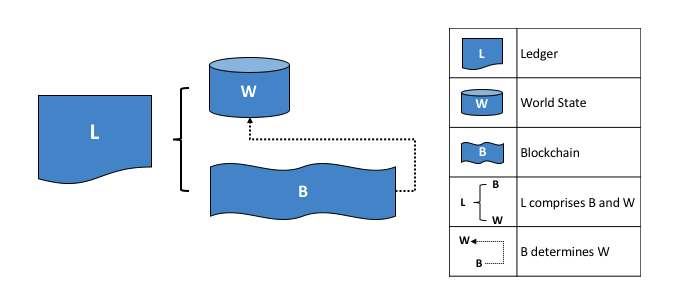
\includegraphics[width=16cm]{ledgerdiagram1.png}
  \caption{An abstract of the Fabric Ledger \cite{fabledger}}
  \label{fabricLedger}
\end{figure}

Physically, the blockchain is always implemented as a file, in contrast to the world state. This is a reasonable design choice as the set of operations on the blockchain data structure is heavily biased towards small limited number. Appending to the end of the blockchain is the primary operation, querying is currently infrequent operation because of the WS. 

\subsubsection{Blocks and their structure}

Figure \ref{fabricBlock} shows how the blockchain is structured and their graphical representation. 

\begin{figure}[h]
\centering
  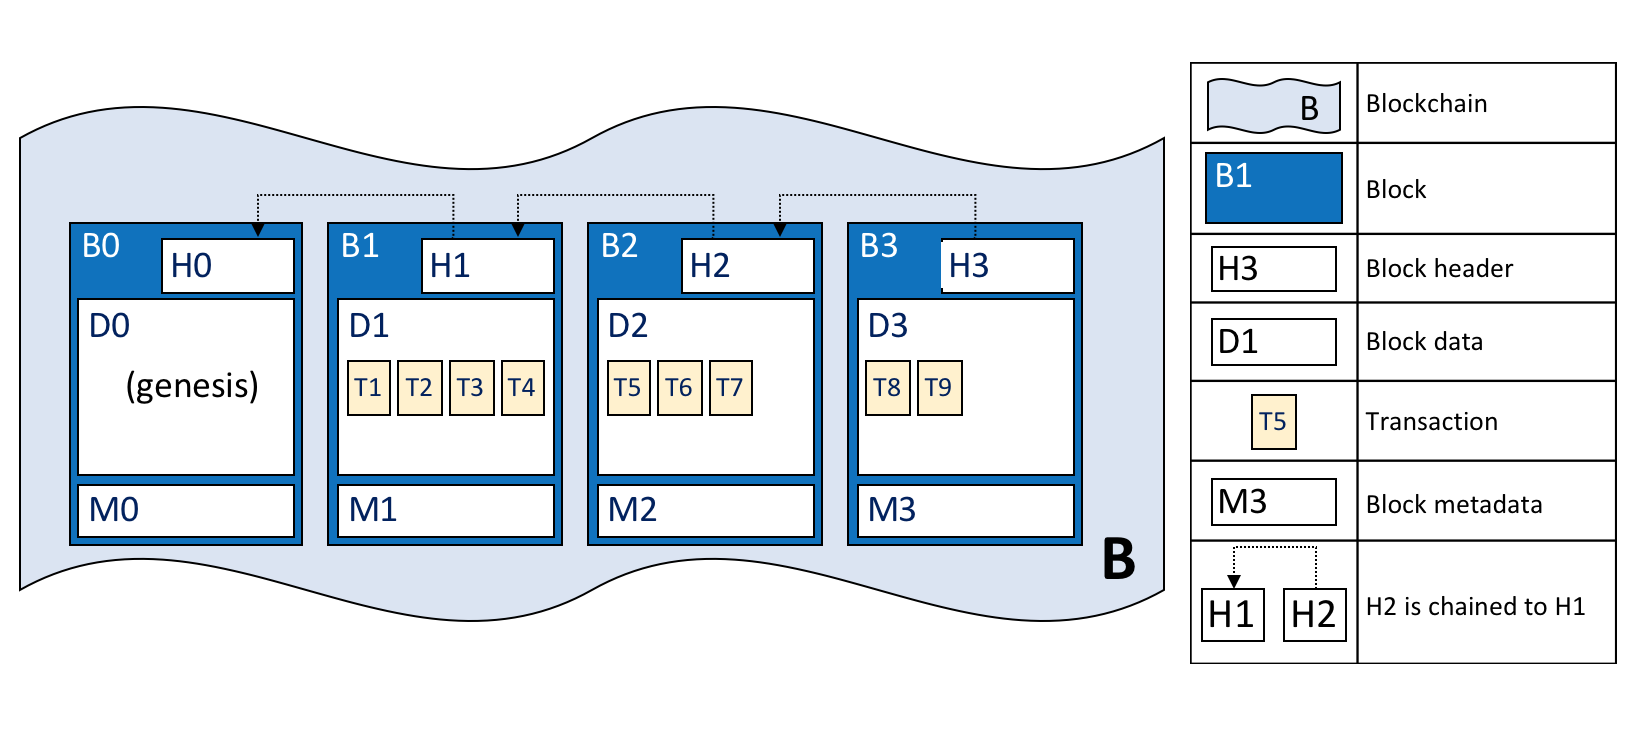
\includegraphics[width=16cm]{ledgerdiagram2.png}
  \caption{An graphical representation of the block \cite{fabledger}}
  \label{fabricBlock}
\end{figure}

\begin{itemize}
\item Block header - consists of three fields:
	\begin{itemize}
	\item Block number - integer, at 0 is the genesis block, increased by one for every new block that is appended to the blockchain
	\item Current block hash - hash of all the transactions contained in the current block
	\item Previous block hash - copy of the hash from the previous block
	\end{itemize}	 
\item Block data - contains a list of transactions arranged in order of appending.
\item Block metadata - contains the time when the block was written as well as, the public key, certificate and signature of the block writer. 
\item Transactions
	\begin{itemize}
	\item Transaction header - captures the essential data about the transaction like name of the chaincode and its version. 
	\item Signature - is being generated only by the user’s private key. The field is used to check that the transaction details have not been changed.
	\item Proposal - encodes input parameters supplied by the user via an application to provide them to the chaincode which creates creates the proposed ledger update. But before the proposed transaction is being added to the blockchain it first has to be verified and validated by the \textit{endorsing peers} which are discussed in the following subsection.
	\item Response - captures the before and after values of the world state, as a read-write set. It’s the output of a chaincode (smart contract), if the transaction is successfully validated, the response will be applied to the ledger to update the world state. 
	\item Endorsements - Although there is only one transaction response, there are multiple endorsements from different \textit{organisations}.If there are not enough endorsements, specified in the transaction verification process, the response would not match the needed number and the transaction will be rejected as invalid and will not update the world state.  
	\end{itemize}
\end{itemize}

\subsection{Channel}
In Ethereum or Bitcoin, when someone joins the network, they are connecting to the blockchain. That being just one ledger starting from genesis block. Every participant has all blocks or just the headers, however, the important note is that everybody keep information from the same blockchain.

	Hyperledger Fabric, contrary to the blockchains above, can have several different ledgers in one network. Since it is build with the premise of business, having several ledgers in a network is beneficial. It is possible, because the ledger is owned by a channel. A channel is like a communication channel, it is the mechanism by which different organizations are interacting between each other. Those interactions are append on the immutable ledger. 
	
What’s more, every channel is having its own business logic, chaincode installed. So a network, depending on the use case, can have one channel with all business partners, one channel with all end users, and several other channels with specific business partners and end users. And all of them can have different chaincodes or the same, depending on the case and requirements of the system.

All peers from a channel have the same ledger. What’s more a peer can have multiple ledgers,hence multiple instances of different chaincode. However, those ledgers are completely different and cannot interact between each other.


\section{Fabric Consensus}
\label{fabricConsensus}
The consensus in fabric is broken out into three phases: Endorsement, Ordering and Validation

\subsection{Endorsement}
Endorsement is driven by policy (m out of n signatures) upon which participants endorse a transaction.

	This phase starts with client application sending transaction proposal. A transaction proposal is an action that will change the state of one or more assets in the ledger. The endorsing peers are taking this proposal and simulate it into the network. The transaction has been signed with the result of the simulation. Depending on the policy, which is defined upon installation of the chaincode, there will be a number of signatures needed before the transaction to proceed into the block. If the policy is not fulfilled then the transaction is going to be rejected.
	    
	Now, at this point, nothing in the ledger is changed. Many different transaction proposals can be taken and put against the current ledger to check out whether the transaction is going to be valid or rejected. While it is done with the premise of scalability, this parallel validation is introducing one problem. 
	
	If there are two transactions being validated that update the state of the same asset, then they will be voted both valid from the endorsing peers. However, once the transactions are being sent to the next phase, the ordering, one of them will fail. Upon batching the transactions they are put into order. Depending on that order, what happens to be second transaction is going to fail.

\subsection{Ordering}
Ordering phase will get the endorsed transaction and agrees to the order to be committed to the ledger.

The ordering phase or service, consists of cluster of orderer nodes. They are receiving the transactions. Batch the transactions into a block. An important event occurs here, that once a transaction is put into the block, it it said to be final. This means that the position of the transaction in the ledger is immutable. The order is consistent and strict. Finally, the blocks are distributed to the committing peers.
	
	Note, the order of the transactions is not necessarily as in the order of the transactions send to the node. This is important, because once the batch is done, some of the transactions may be rejected. It can happen due to the fact that two transactions may have tried to change the same resource, and only one change can happen per block. When transaction proposals enter the network, the endorsers are simulating them in a parallel manner, against the current ledger. So, both transactions will be looking at the same state of the asset they want to change. Both of them can be valid, however, the first that gets to be put in the order batch is the one that is going to make the change in the blockchain and world state. The second is going to be rejected.
	
Batches are defined mainly by two factors. The first is the time to wait before a block is being generated. The waiting starts after the first transaction is received and can finish on the time specified or before that. For a block to be generated before the end of the time set, the block’s size had to reach its limit. If the configuration is done so that 10 transactions can be put into a block, and 2 seconds to be time set, then there are two cases. First - have a block in 1 second with 10 transactions. Second - have a block with less than 10 transactions after 2 seconds. The configuration can be found in confingtx.yaml. Will be discussed in more detail in the configuration section. (12 min [20] )

	So in order to effectively avoid invalid transactions due to two transactions updating the same resource, the configuration of generating the blocks have to be well-thought for the specific system. 
	
There are several types of ordering mechanisms implemented in Fabric. They are all pluggable, so the engineers of the network can try with one of them and then go to the other, simply to see which one will be most efficient for the case: 
\begin{itemize}
\item SOLO - involves a single ordering node, single point of failure. It is very fast, but unreliable for real data, which makes it the perfect mechanism in developing stage. 
\item Kafka - based on Apache Kafka, high-throughput, low-latency platform. Crash fault-tolerant solution. 
\item PBFT - practical byzantine fault tolerant mechanism. It is both crash fault and byzantine fault tolerant, meaning it can reach an agreement even in the presence of malicious or faulty nodes. Slow, but secure.
\end{itemize}
According to a IBM paper \cite{cachin2016architecture}, PBFT is the most used one in production, however, due to the pluggable design, depending on the network, it can be changed with Kafka or a future solution.

Usually, since the first and the third steps are always the same, people would refer to Fabric consensus just as the name of the ordering mechanism.

\subsection{Validation}

Validation - takes a block of ordered transactions and validates the correctness of the result. 
	The moment a committer node receives the new block, it starts checking every transaction and the transaction result from the endorsing peers. This check is against the endorsement policy. Here is the moment where if two transactions are trying to change the one asset, the second fails. However, instead of returning the whole block, the faulty transaction is just being labeled as \textit{invalid}. The committer updates the ledger. Lastly, asynchronously returns to the user/app that the transaction is successful or not. 

\section{Fabric's configuration}

\section{Hyperledger Composer}
\label{hplComposer}

%%%%%%%%%%%%%%%%%%%%%%%%%%%%%%%%%%  Use Case  %%%%%%%%%%%%%%%%%%%%%%%%%%%%%%%%%
\chapter{Use case}
\label{usecase}

%%%%%%%%%%%%%%%%%%%%%%%%%%%%%%%%%%  User Manual  %%%%%%%%%%%%%%%%%%%%%%%%%%%%%%%%%

\chapter{User Manual}
\label{usermanual}


\section{Step one}
\label{stepOne}
	 

%%%%%%%%%%%%%%%%%%%%%%%%%%%%%%%%%%  Conclusion %%%%%%%%%%%%%%%%%%%%%%%%%%%%%%%%%

\chapter{Conclusion}

\label{conclusion}

\section{Evaluation}

\label{conclusion-evaluation}

If you do not have a separate chapter on testing, explain here in detail how you
went about systematically testing your system. If appropriate, also include
end users in your testing. Summarise your main results, and explain how you have
advanced the state-of-the-art. Stand back and evaluate what you have achieved
and how well you have met the objectives. Evaluate your achievements against the
objectives stated in section~\ref{introduction-objectives}. Demonstrate that you
have tackled the project in a professional manner.

\section{Future Work}

\label{conclusion-future}

Explain any limitations in your results and how things might be improved.
Discuss how your work might be developed further. Reflect on your results in
isolation and in relation to what others have achieved in the same field. This
self-analysis is particularly important. You should give a critical evaluation
of what went well, and what might be improved.

% Citations

\bibliographystyle{abbrv}

\bibliography{ref}

% Appendixes

\appendix


\end{document}
